% Options for packages loaded elsewhere
% Options for packages loaded elsewhere
\PassOptionsToPackage{unicode}{hyperref}
\PassOptionsToPackage{hyphens}{url}
\PassOptionsToPackage{dvipsnames,svgnames,x11names}{xcolor}
%
\documentclass[
  french,
  9pt,
  a4paper,
  DIV=11,
  twoside=semi]{scrreprt}
\usepackage{xcolor}
\usepackage{amsmath,amssymb}
\setcounter{secnumdepth}{3}
\usepackage{iftex}
\ifPDFTeX
  \usepackage[T1]{fontenc}
  \usepackage[utf8]{inputenc}
  \usepackage{textcomp} % provide euro and other symbols
\else % if luatex or xetex
  \usepackage{unicode-math} % this also loads fontspec
  \defaultfontfeatures{Scale=MatchLowercase}
  \defaultfontfeatures[\rmfamily]{Ligatures=TeX,Scale=1}
\fi
\usepackage{lmodern}
\ifPDFTeX\else
  % xetex/luatex font selection
\fi
% Use upquote if available, for straight quotes in verbatim environments
\IfFileExists{upquote.sty}{\usepackage{upquote}}{}
\IfFileExists{microtype.sty}{% use microtype if available
  \usepackage[]{microtype}
  \UseMicrotypeSet[protrusion]{basicmath} % disable protrusion for tt fonts
}{}
\usepackage{setspace}
\makeatletter
\@ifundefined{KOMAClassName}{% if non-KOMA class
  \IfFileExists{parskip.sty}{%
    \usepackage{parskip}
  }{% else
    \setlength{\parindent}{0pt}
    \setlength{\parskip}{6pt plus 2pt minus 1pt}}
}{% if KOMA class
  \KOMAoptions{parskip=half}}
\makeatother
% Make \paragraph and \subparagraph free-standing
\makeatletter
\ifx\paragraph\undefined\else
  \let\oldparagraph\paragraph
  \renewcommand{\paragraph}{
    \@ifstar
      \xxxParagraphStar
      \xxxParagraphNoStar
  }
  \newcommand{\xxxParagraphStar}[1]{\oldparagraph*{#1}\mbox{}}
  \newcommand{\xxxParagraphNoStar}[1]{\oldparagraph{#1}\mbox{}}
\fi
\ifx\subparagraph\undefined\else
  \let\oldsubparagraph\subparagraph
  \renewcommand{\subparagraph}{
    \@ifstar
      \xxxSubParagraphStar
      \xxxSubParagraphNoStar
  }
  \newcommand{\xxxSubParagraphStar}[1]{\oldsubparagraph*{#1}\mbox{}}
  \newcommand{\xxxSubParagraphNoStar}[1]{\oldsubparagraph{#1}\mbox{}}
\fi
\makeatother


\usepackage{longtable,booktabs,array}
\usepackage{calc} % for calculating minipage widths
% Correct order of tables after \paragraph or \subparagraph
\usepackage{etoolbox}
\makeatletter
\patchcmd\longtable{\par}{\if@noskipsec\mbox{}\fi\par}{}{}
\makeatother
% Allow footnotes in longtable head/foot
\IfFileExists{footnotehyper.sty}{\usepackage{footnotehyper}}{\usepackage{footnote}}
\makesavenoteenv{longtable}
\usepackage{graphicx}
\makeatletter
\newsavebox\pandoc@box
\newcommand*\pandocbounded[1]{% scales image to fit in text height/width
  \sbox\pandoc@box{#1}%
  \Gscale@div\@tempa{\textheight}{\dimexpr\ht\pandoc@box+\dp\pandoc@box\relax}%
  \Gscale@div\@tempb{\linewidth}{\wd\pandoc@box}%
  \ifdim\@tempb\p@<\@tempa\p@\let\@tempa\@tempb\fi% select the smaller of both
  \ifdim\@tempa\p@<\p@\scalebox{\@tempa}{\usebox\pandoc@box}%
  \else\usebox{\pandoc@box}%
  \fi%
}
% Set default figure placement to htbp
\def\fps@figure{htbp}
\makeatother


% definitions for citeproc citations
\NewDocumentCommand\citeproctext{}{}
\NewDocumentCommand\citeproc{mm}{%
  \begingroup\def\citeproctext{#2}\cite{#1}\endgroup}
\makeatletter
 % allow citations to break across lines
 \let\@cite@ofmt\@firstofone
 % avoid brackets around text for \cite:
 \def\@biblabel#1{}
 \def\@cite#1#2{{#1\if@tempswa , #2\fi}}
\makeatother
\newlength{\cslhangindent}
\setlength{\cslhangindent}{1.5em}
\newlength{\csllabelwidth}
\setlength{\csllabelwidth}{3em}
\newenvironment{CSLReferences}[2] % #1 hanging-indent, #2 entry-spacing
 {\begin{list}{}{%
  \setlength{\itemindent}{0pt}
  \setlength{\leftmargin}{0pt}
  \setlength{\parsep}{0pt}
  % turn on hanging indent if param 1 is 1
  \ifodd #1
   \setlength{\leftmargin}{\cslhangindent}
   \setlength{\itemindent}{-1\cslhangindent}
  \fi
  % set entry spacing
  \setlength{\itemsep}{#2\baselineskip}}}
 {\end{list}}
\usepackage{calc}
\newcommand{\CSLBlock}[1]{\hfill\break\parbox[t]{\linewidth}{\strut\ignorespaces#1\strut}}
\newcommand{\CSLLeftMargin}[1]{\parbox[t]{\csllabelwidth}{\strut#1\strut}}
\newcommand{\CSLRightInline}[1]{\parbox[t]{\linewidth - \csllabelwidth}{\strut#1\strut}}
\newcommand{\CSLIndent}[1]{\hspace{\cslhangindent}#1}

\ifLuaTeX
\usepackage[bidi=basic]{babel}
\else
\usepackage[bidi=default]{babel}
\fi
% get rid of language-specific shorthands (see #6817):
\let\LanguageShortHands\languageshorthands
\def\languageshorthands#1{}


\setlength{\emergencystretch}{3em} % prevent overfull lines

\providecommand{\tightlist}{%
  \setlength{\itemsep}{0pt}\setlength{\parskip}{0pt}}



 


\makeatletter
\@ifpackageloaded{caption}{}{\usepackage{caption}}
\AtBeginDocument{%
\ifdefined\contentsname
  \renewcommand*\contentsname{Table des matières}
\else
  \newcommand\contentsname{Table des matières}
\fi
\ifdefined\listfigurename
  \renewcommand*\listfigurename{Graphiques}
\else
  \newcommand\listfigurename{Graphiques}
\fi
\ifdefined\listtablename
  \renewcommand*\listtablename{Tableaux}
\else
  \newcommand\listtablename{Tableaux}
\fi
\ifdefined\figurename
  \renewcommand*\figurename{Graphique}
\else
  \newcommand\figurename{Graphique}
\fi
\ifdefined\tablename
  \renewcommand*\tablename{Tableau}
\else
  \newcommand\tablename{Tableau}
\fi
}
\@ifpackageloaded{float}{}{\usepackage{float}}
\floatstyle{ruled}
\@ifundefined{c@chapter}{\newfloat{codelisting}{h}{lop}}{\newfloat{codelisting}{h}{lop}[chapter]}
\floatname{codelisting}{Listing}
\newcommand*\listoflistings{\listof{codelisting}{Liste des Listings}}
\makeatother
\makeatletter
\makeatother
\makeatletter
\@ifpackageloaded{caption}{}{\usepackage{caption}}
\@ifpackageloaded{subcaption}{}{\usepackage{subcaption}}
\makeatother
\usepackage{bookmark}
\IfFileExists{xurl.sty}{\usepackage{xurl}}{} % add URL line breaks if available
\urlstyle{same}
\hypersetup{
  pdftitle={Modéliser les mobilités à une échelle fine},
  pdfauthor={Maxime Parodi (xavier.timbeau@sciencespo.fr); Xavier Timbeau (xavier.timbeau@sciencespo.fr)},
  pdflang={fr},
  colorlinks=true,
  linkcolor={blue},
  filecolor={Maroon},
  citecolor={Blue},
  urlcolor={Blue},
  pdfcreator={LaTeX via pandoc}}


%%% title.tex we use to call other packages. Because this works
\usepackage{titlepic}
\usepackage{titling}
\usepackage{graphicx}
\usepackage{fontspec}
\usepackage{placeins}
\usepackage{graphbox}
\usepackage{tikz}
\usepackage{geometry}
\usepackage{xcolor}
\usepackage{amsmath}
\usepackage[some]{background}
\usepackage{lipsum}
\usepackage{caption}
\usepackage{datetime}
\usepackage{xstring}
\usepackage{blindtext}
\usepackage{scrlayer-scrpage}

\setmainfont{OpenSans}[
  UprightFont = {*-Regular},
  BoldFont = {*-Bold},
  BoldItalicFont = {*-BoldItalic},
  ItalicFont = {*-Italic},
  Path = {_extensions/ofce/wp/OpenSans/},
  Extension = {.ttf}
]
\setsansfont{OpenSans}[
  UprightFont = {*-Regular},
  BoldFont = {*-Bold},
  BoldItalicFont = {*-BoldItalic},
  ItalicFont = {*-Italic},
  Path = {_extensions/ofce/wp/OpenSans/},
  Extension = {.ttf}
]

\def\getYear#1{\StrLeft{#1}{4}}
\def\getMonth#1{\StrMid{#1}{6}{7}}
\def\getDay#1{\StrRight{#1}{2}}

\def\jolimois#1{\monthname{\getMonth{#1}}}

\definecolor{quarto-callout-color}{HTML}{eeeeee}
\definecolor{quarto-callout-tip-color}{HTML}{dddddd}
\definecolor{quarto-callout-tip-color-frame}{HTML}{eeeeee}

\clearpairofpagestyles

\KOMAoptions{headsepline=true}

\pagestyle{scrheadings}
\setkomafont{pageheadfoot}{\small}

\lofoot*{\thepage}
\refoot*{\thepage}
\begin{document}



\definecolor{ofcepbbleu}{RGB}{1, 97, 131}
\definecolor{ofcerouge}{RGB}{198, 45, 43}
\definecolor{scporouge}{RGB}{231, 0, 26}

\begin{titlepage}
  \backgroundsetup{
    scale=1,
    angle=0,
    opacity=1,
    contents={
  \begin{tikzpicture}[remember picture,overlay]
    \useasboundingbox (0,0) rectangle(\the\paperwidth,\the\paperheight);
      \node [anchor = center] at (-2.875-5.25,12.5) {\includegraphics[width=2.5cm]{\_extensions/ofce/note/logos/ofce\_m.png}};
      \node [anchor = center] at (-2.875-5.25,-12.75){
\includegraphics[width=2.5cm]{\_extensions/ofce/note/logos/sciencespo.png}};
      \node [anchor = east] at (8.5,-11.5){\textcolor{black}{Publié le : 2025-09-22}};
            \end{tikzpicture}
  }
}
\BgThispage

\hspace{4cm}
\begin{minipage}{12.5cm}
  \vspace{5cm}
  \begin{flushleft}
    \begin{spacing}{2.5}
      \textcolor{scporouge}{\Huge\textbf{\textsf{Modéliser les mobilités
à une échelle fine}}}
    \end{spacing}
    \vspace{20mm}
  \end{flushleft}
  
    
   \textbf{Maxime Parodi (xavier.timbeau@sciencespo.fr)}
   
   \textbf{Xavier Timbeau (xavier.timbeau@sciencespo.fr)}
  % by-author
 \end{minipage}


\end{titlepage}

\setstretch{1.25}
\chapter{MEAPS\,: de l'accessibilité au
trajets}\label{meaps-de-laccessibilituxe9-au-trajets}

L'accessibilité (aux opportunités, cf. Bousquet, Caubel, et Chevereau
(2015)) est une notion féconde. Développée après guerre, par Hansen
(1959) elle est au cœur de l'analyse des réseaux de transports et de la
mobilité. En France par exemple, Poulit (2005) et Koenig (1980) ont
utilisé largement ce concept aux Ponts et Chaussées, dans l'analyse des
réseaux routiers.

Nous avons développé une méthode pour calculer l'accessibilité à une
échelle géographique fine (carreau INSPIRE 200m\$\times\$200m), pour de
nombreuses catégories d'opportunités (emploi, commerces, etc\ldots) et
pour différents modes de transport (à pied, en transport en commun, en
vélo ou en voiture).

\pandocbounded{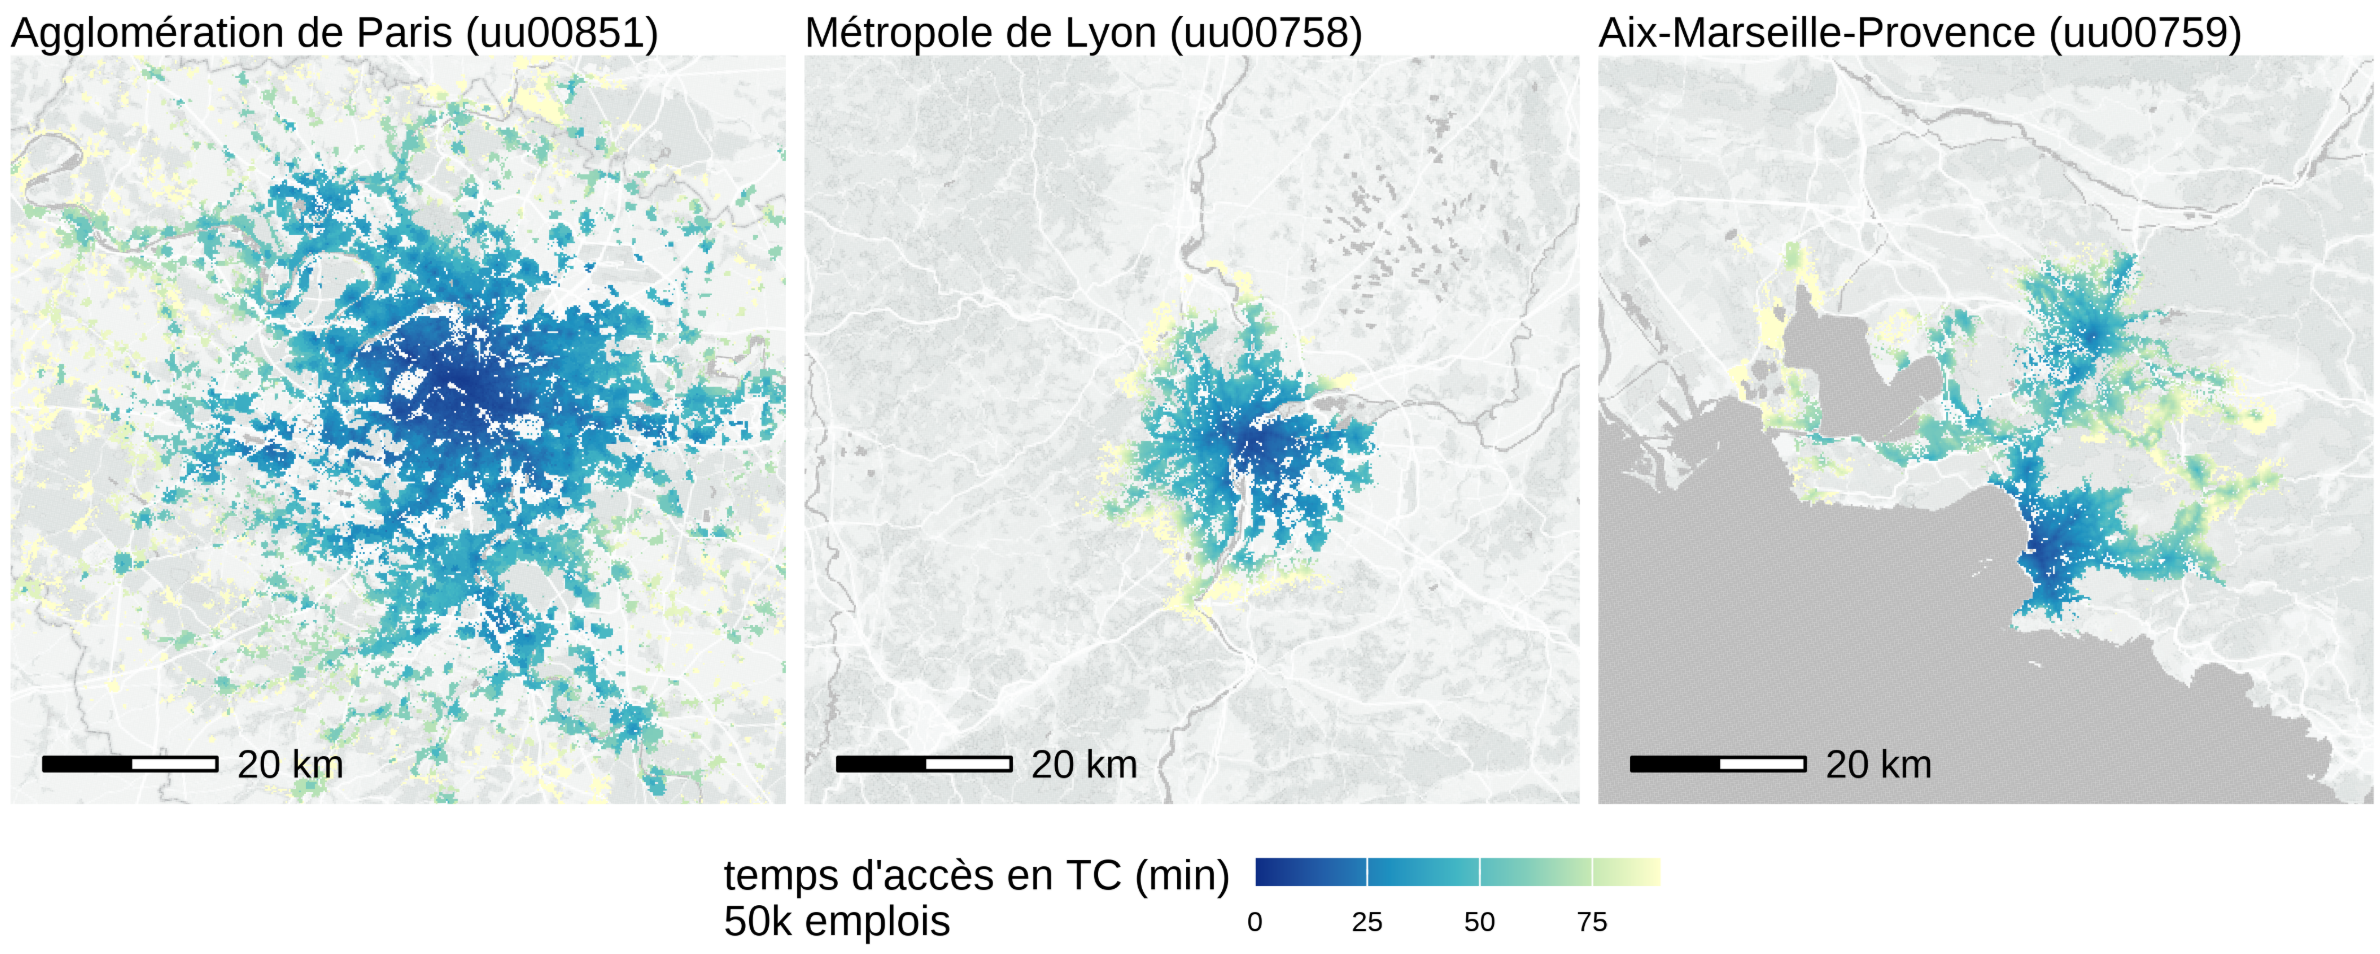
\includegraphics[keepaspectratio]{images/clipboard-3675797071.png}}

Deux difficultés d'ordre pratiques ont été résolues\,: l'utilisation
d'informations géographiques pertinentes pour la résolution choisie et
la volumétrie de calcul impliquée. Par exemple, pour la métropole
d'Aix-Marseille-Provence, plus d'un milliard de distances sont calculées
entre chaque paire origine-destination. La résolution employée, combinée
aux données fines, permet de construire des scénarios pour représenter
par exemple l'impact d'un nouveau réseau comme le Grand Paris Express.

\begin{center}
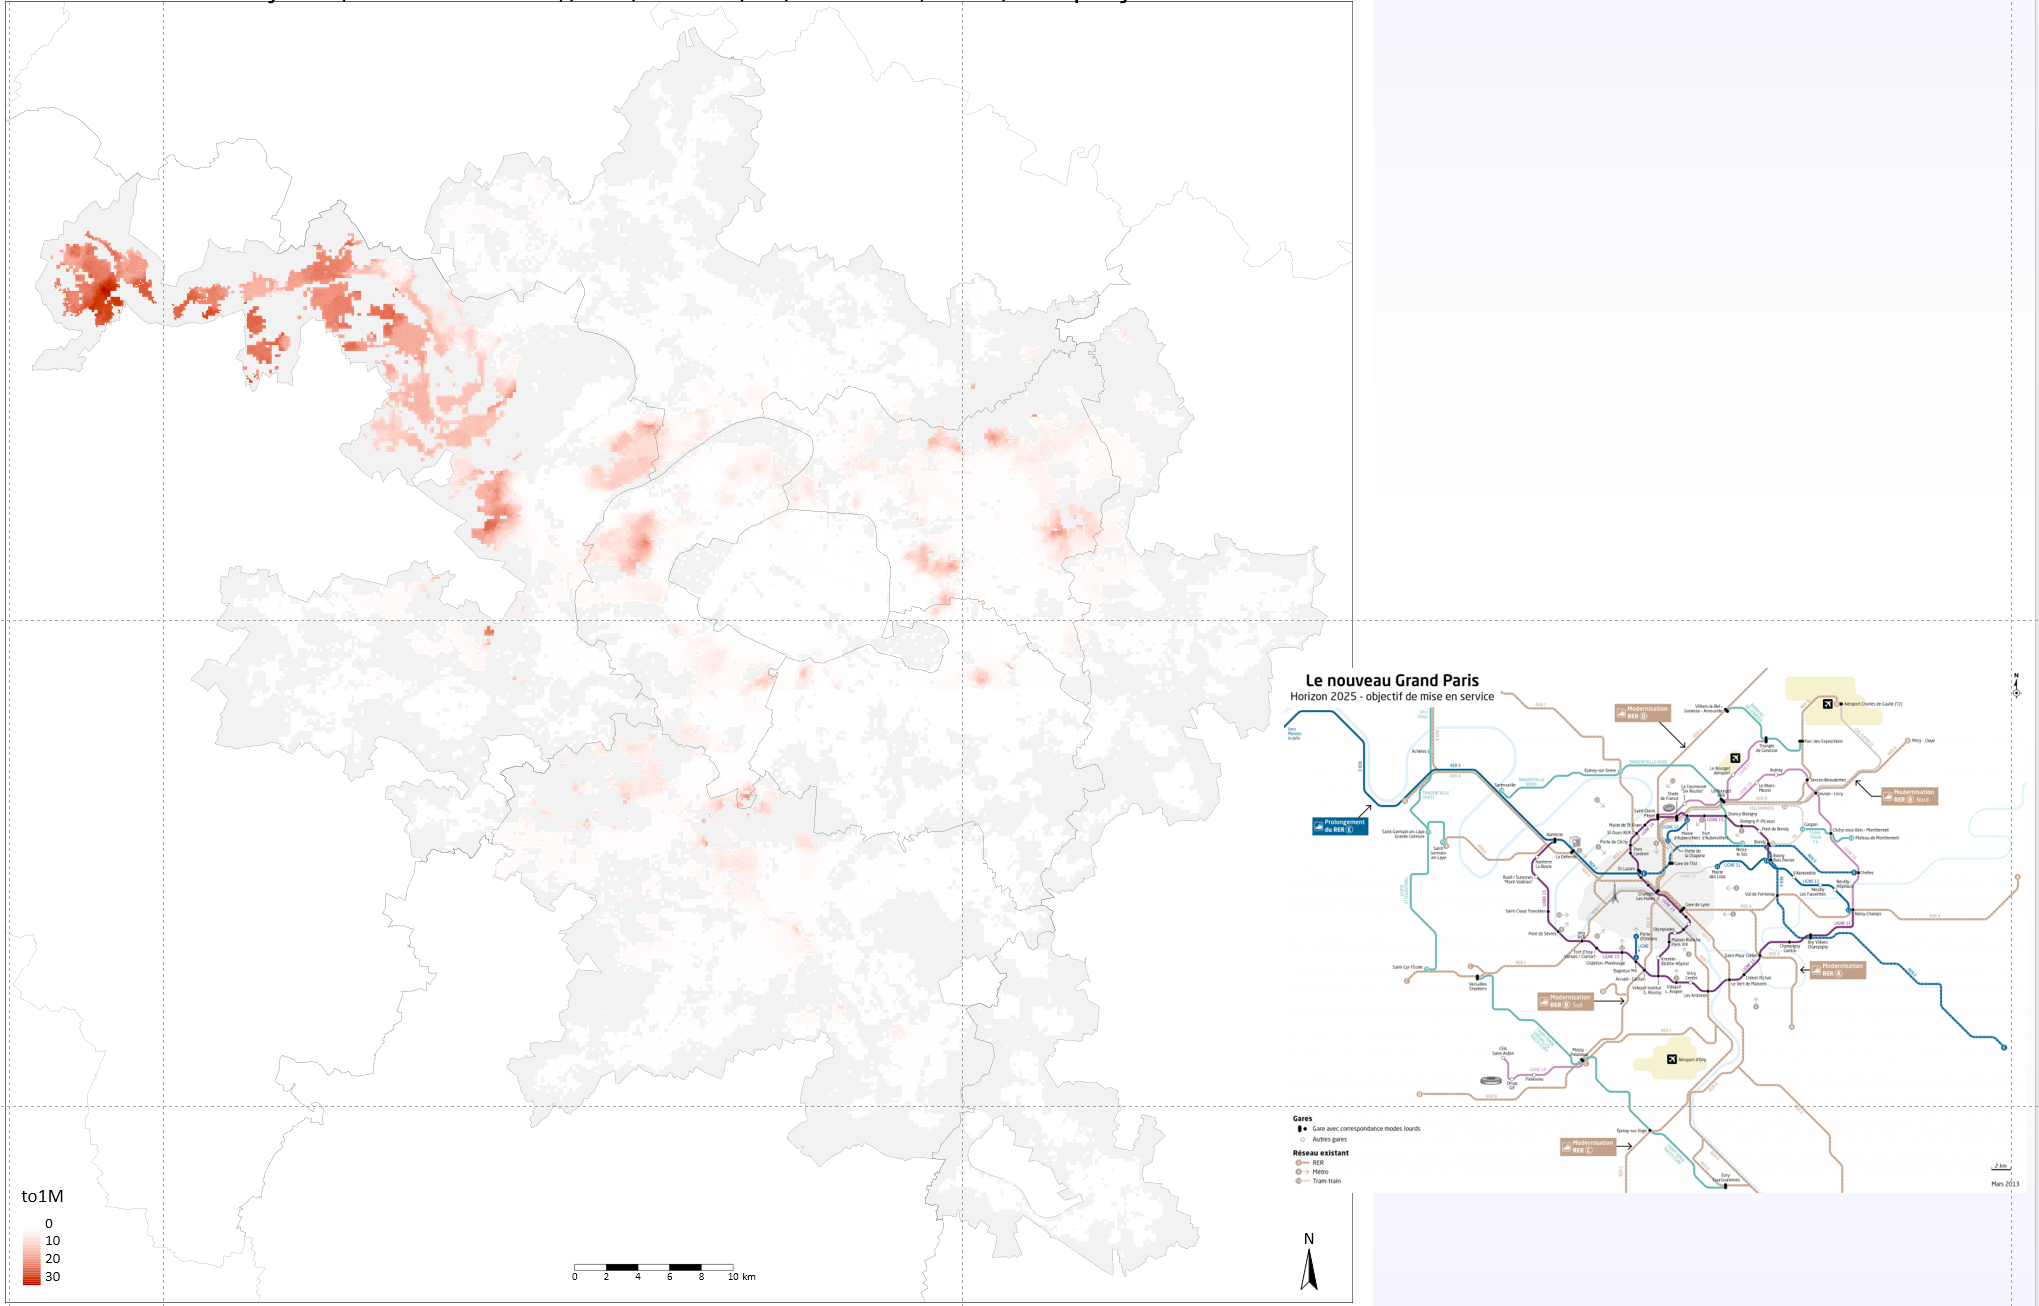
\includegraphics[width=5.3125in,height=\textheight,keepaspectratio]{images/clipboard-3092760633.png}
\end{center}

L'accessibilité quantifie un potentiel. Pour aller plus loin, nous avons
développé un modèle théorique (Parodi et Timbeau 2023) qui remplace le
modèle gravitaire (affecter des flux en fonction de distances ou de
coûts généralisés), en permettant de prendre en compte la double
concurrence des individus voisins pour les mêmes opportunités
(lorsqu'elles ont une capacité finie) et, réciproquement, la concurrence
des opportunités pour les individus (lorsque les opportunités doivent
être remplies, e.g.~des emplois). Associé à cette modélisation
originale, nous avons développé des méthodes d'estimation qui permettent
d'ajuster le modèle sur des données comportementales comme l'enquête
mobilité des personnes (Parodi et Timbeau 2024b).

Ces modèles, qui mobilisent des sources de données disparates de façon
cohérente, sont des outils efficaces pour traiter des questions de forme
urbaine. Quelles sont les conséquences de la répartition spatiales des
emplois et des logements, reliés par des réseaux de transport sur le
bilan carbone mobilité d'un territoire\,? Comment la densification des
logements, le dimensionnement du réseau de transport ou les politiques
publiques d'incitation au vélo peuvent modifier ce bilan\,? Au delà du
bilan carbone, quel est le coût de la mobilité et comment se
combine-t-il au coût du logement pour analyser les tensions sociales
d'un territoire\,?

Dans Parodi et Timbeau (2024a) nous tirons ainsi une conclusion
importante\,: la littérature en économie urbaine a conclut, de façon
convaincante et robuste, que le lien entre densité et émissions (de tout
genre) était positif (ce qui est conforme à l'intuition) mais très
faible (ce qui est ennuyeux). Ainsi, pour significativement réduire les
émissions (disons de 30\%), il faudrait augmenter la densité de 300\% ce
qui paraît impossible à faire tant l'effort individuel ou collectif
demandé est considérable. Pourtant, nous arguons que la question est mal
posée. La densité n'est pas une notion homogène et accroître la densité
«\,près\,» des emplois n'a pas le même impact que plus loin, dès lors
qu'on sait définir correctement le proche et le lointain. La prise en
compte explicite des co-distributions spatiales des emplois et des
logements permet de donner à ces éléments un contenu précis.

Le travail empirique réalisé à la Rochelle permet de quantifier ce
contenu, et d'éclairer la conclusion consensuelle sur le lien entre la
densité urbaine et les émissions de CO\textsubscript{2} sous un jour
nouveau, au moins à la Rochelle\,: on peut par une localisation bien
définie de l'accroissement de la densité être plus efficace. Au lieu
d'une augmentation de la densité de 300\% il suffit d'une augmentation
de la densité (moyenne) de 30\%, ce qui en fait un obstacle bien plus
facile à franchir.

\begin{center}
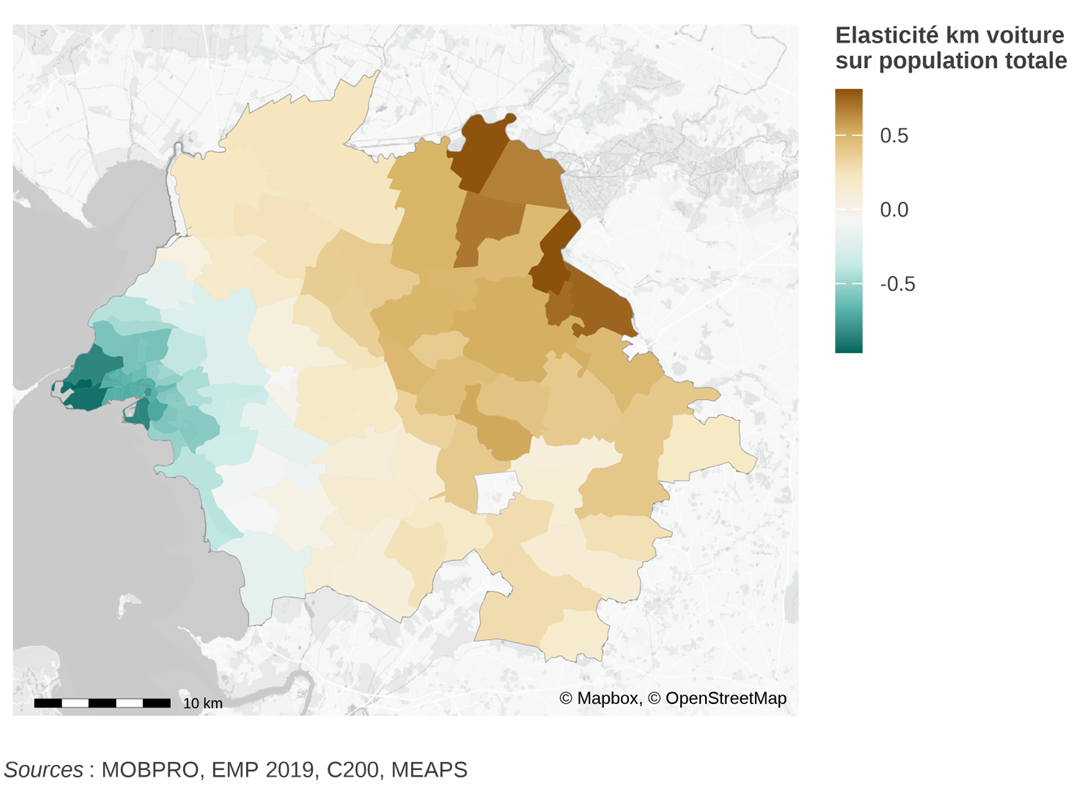
\includegraphics[width=6.42708in,height=\textheight,keepaspectratio]{images/clipboard-1456870736.png}
\end{center}

Pourquoi se limiter à la Rochelle ou Marseille\,? Comment rendre plus
solides les analyses empiriques proposées\,? Comment développer les
applications\,? C'est le sens du projet proposé\,: le travail théorique
et empirique peut être généralisé à de nombreux territoires, il a été
appliqué et expérimenté sur quelques exemples\,: La Rochelle,
Clermont-Ferrand, Aix-Marseille-Provence. La généralisation à l'ensemble
des agglomérations françaises, voire européennes, est envisageable pour
un coût bien inférieur, mais non nul, à l'investissement initial.

\chapter{Le projet}\label{le-projet}

L'ambition est donc de\,:

\begin{enumerate}
\def\labelenumi{\arabic{enumi}.}
\item
  \textbf{approfondir le travail empirique de recherche avec les données
  issues de Fluxvision}. L'analyse a été menée jusqu'à maintenant en
  utilisant MOBPRO comme source de matrice origine destination. La
  modélisation permet d'intrapoler à une échelle plus fine
  (200m\$\times\$200m) que la résolution de MOBPRO
  (commune/arrondissement à commune/arrondissement) en incorporant
  d'autres données (les comportements de l'Enquête Mobilité par
  exemple). L'utilisation des données de Fluxvision et plus
  particulièrement les matrices origines destinations dérivées dans les
  travaux financés par Transdev sont une piste majeure. Il y est plus
  difficile d'identifier les motifs ou les catégories sociales des
  navetteurs, mais les données sont plus riches et sans doute plus
  robustes parce qu'elles en sont pas déclaratives, ne résument pas une
  année, reposent sur un échantillon massif, permettent d'approcher les
  multi-destinations, les schémas temporels de l'intra-semaine aux
  variations saisonnières, ou aux périodes particulières.\\
  Elles doivent aussi permettre d'évaluer les mobilités difficiles à
  mesurer comme les itinérants. De plus, les données de \emph{la France
  Habitée} (Lévy et al. 2023) peuvent permettre de définir une
  opportunité \emph{synthétique}, alternative à l'approche
  d'identification directe des opportunités suivies jusque là, qui
  permettra d'approcher l'attractivité révélée et peut être les aspects
  de mixité sociale (les lieux visités par des individus venant d'IRIS
  variés dans leur compositions sociales par exemple). Une phase de
  recherche importante est à envisagée parce que les données Fluxvision
  et dérivées ne distinguent pas les motifs. Elles font apparaître des
  phénomènes non analysés et peuvent mal mesurer ceux qui l'ont déjà
  été. Nous proposons une phase initiale de la recherche sur la
  métropole d'Aix-Marseille-Provence, pour laquelle nous disposons de
  nombreux éléments de comparaison ainsi que d'une
  EMC\textsuperscript{2}. Une fois l'analyse et l'utilisation des
  données de Fluxvision et leurs transformations stabilisées, on peut
  entreprendre la généralisation aux 50 plus grandes aglomérations.
\item
  \textbf{produire des éléments les plus robustes possibles sur un
  ensemble de territoires} -- les 50 premières agglomérations françaises
  (ou de plus de 200\,000 résidents) dans un premier temps\,-- pour
  alimenter le débat sur l'aménagement, dans ses dimensions
  environnementales mais aussi sociales. Ces éléments sont à l'échelle
  fine du carreau 200m\$\times\$200m, appuyés sur les données du
  recensement MOBPRO et de Fluxvision (voir 1.). Ces analyses sont dans
  la prolongation de l'analyse des flux de mobilités pour la Rochelle ou
  \hyperref[0]{Aix-Marseille-Provence} -- où l'analyse a été étendue du
  seul motif mobilité professionnelle à l'ensemble des motifs en
  utilisant l'EMC\textsuperscript{2}. Les données Fluxvision peuvent
  apporter une meilleure robustesse par une mesure fréquente et
  exhaustive. Les matrices de flux permettent de générer des cartes
  d'émissions de CO\textsubscript{2} imputées aux résidents et sont un
  bon résumé de la structure des territoires. Le principe est celui de
  la diffusion en source ouverte d'un certain nombre d'informations, à
  affiner en fonction des objectifs (de prestations autour de ces
  concepts, par exemple des simulations à partir du modèle de scénarios,
  des analyses plus fines des comportements, l'analyse multi-motifs si
  EMC\textsuperscript{2}) et des possibilités de réutilisation des
  données sources (par exemple, les analyses sociologiques fines
  demandent l'utilisation de Fidéli, mais limitent les rediffusions).
\item
  \textbf{analyser les formes urbaines à partir des données produites}.
  En disposant de cartes CO\textsubscript{2} fines, agrégées en
  indicateurs à définir, on peut procéder à une classification des
  formes urbaines ou procéder par régression et corrélation multivariée
  avec d'autres variables localisées pour synthétiser l'information
  géographique sous jacente en une analyse pertinente. Il existe
  plusieurs exemples de tentatives de ce type, assez peu convaincantes
  ou opérationnelles au final\,; la possibilité d'articuler distribution
  spatiale des opportunités et des logements ainsi que la capacité à
  prendre en compte les réseaux de transport devrait faire aboutir ce
  type de démarche. Cette analyse compléterait les cartes
  CO\textsubscript{2} locales par une approche globale et synthétique.
  L'analyse peut également intégrer une dimension temporelle. Nous avons
  développé des algorithmes permettant de tenir compte des changements
  d'IRIS et de reprojetter les populations (et les flux MOBPRO) sur un
  découpage fixe dans le temps. L'analyse de la dynamique (par exemple
  vitesse de l'étalement urbain) peut être combinée à des analyses plus
  statitiques. Des projections peuvent être envisagées sur la base des
  tendances identifiées, afin d'appuyer sur la nécessité de modifier le
  paradigme des politiques publiques d'aménagement. L'analyse des formes
  urbaines peut également intégrer des éléments du 2. concernant les
  dimensions socio-économiques.
\item
  \textbf{dérouler des applications des modélisations et des
  transformations des données}. Dans notre démarche, la modélisation
  sert de cadre pour donner extraire de données riches une information
  pertinente. Pour en démontrer la pertinence, il faut pouvoir produire
  des applications. Outre l'analyse des territoires, susceptible par
  exemple d'influencer l'élaboration des schémas de cohérence
  territoriale (SCoT), une application pourrait être le design des
  réseaux de transport. Les modèles développés permettent en effet de
  projeter ce qui se passerait si une ligne de transport en commun (bus,
  tram, train) était ajoutée. Sous l'hypothèse (de moyen terme) que les
  populations ne changent pas, il est possible en effet de partir des
  comportements observés pour estimer le changement modal qui pourrait
  être opérer et de produire une évaluation des projections de flux. La
  méthode tient compte finement des variations de temps de trajet pour
  chaque mode, des ruptures de charges et d'autres éléments (comme le
  multimodal). Elle est une alternative à des modèles de transport
  habituels et, combiné au point 1., elle reposerait sur des données
  nouvelles. Elle pourrait être confronté à des réalisations passées
  pour en valider la portée. D'autres applications sont possibles, comme
  des scénarios d'évolution à l'horizon de 10 ou 20 années.
\end{enumerate}

\chapter{Projets parallèles}\label{projets-paralluxe8les}

Deux projets parallèles à celui-ci valent la peine d'être mentionnés
parce qu'ils peuvent compléter les analyses proposées dans le projet.

\section{Dynamiques urbaines (ODU)}\label{dynamiques-urbaines-odu}

Sur la base des calculs d'accessibilité, et des différents vintages de
MOBPRO, on peut analyser les évolutions des mobilités quotidiennes pour
la mobilité professionnelle sur des périodes de temps de 10 à 20~ans.
Cette comparaison temporelle doit être faite avec soin et elle produit
un ensemble de données riches à mettre en rapport avec les formes
urbaines (point 2.). Les éléments de cette analyse pourrait être
associées à celles ci pour compléter l'offre en source ouverte.

\section{Difficultés de
recrutement}\label{difficultuxe9s-de-recrutement}

En réponse à un Appel à Projet de Recherche lancé par le PUCA (BEL),
nous avons proposé une analyse des difficultés de recrutement issues des
données de l'enquête Besoin de Main d'Œuvre et de leur lien avec
l'accessibilité à l'emploi. Pour chaque entreprise interrogée (plus de
2~millions chaque année) nous disposons de sa localisation et nous
pouvons lui associer une mesure de sa distance à l'emploi, de la
quantité d'emplois potentiels accessibles, de la quantité de personnes
en recherche d'emploi, du degré de concurrence entre entreprises
recherchant des emplois. Sur la base de cette association et de la
variance géographique, nous nous proposons de produire une analyse
causale entre difficulté de recrutement et structure spatiale des
logements ou des résidents et des réseaux de transport.

\chapter{Calendrier prospectif et
livrables}\label{calendrier-prospectif-et-livrables}

\pandocbounded{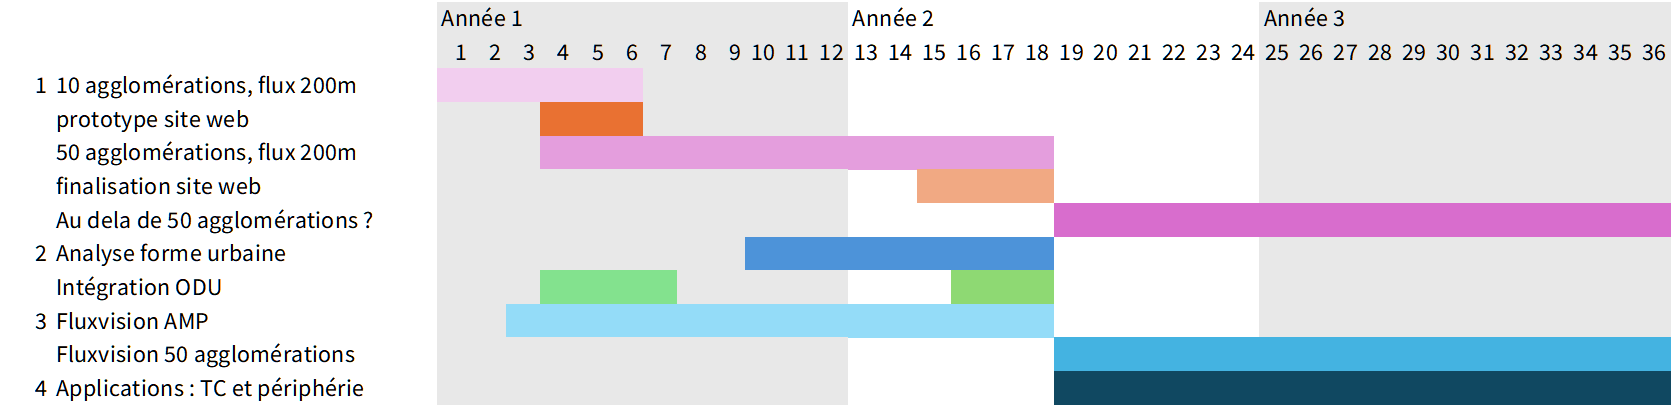
\includegraphics[keepaspectratio]{images/clipboard-1491914023.png}}

La première phase du projet est la reproduction des analyses fines de
bilan CO\textsubscript{2} pour un ensemble d'agglomérations. Le délai de
production est de l'ordre de 12 mois, un premier livrable (site web
présentant les données pour une sous sélection) pouvant être construit
d'ici à 6 mois après le lancement du projet.

Dans un délai de 12 à 18 mois, l'analyse des formes urbaines pourrait
être achevée, publiée sous forme d'un document de travail, et venir
augmenter le site web.

L'utilisation des données de Fluxvision serait concentrée dans un
premier temps sur l'agglomération d'Aix-Marseille-Provence (AMP). C'est
en effet sur ce territoire que notre analyse globale de la mobilité est
la plus aboutie. La disponibilité des données EMC\textsuperscript{2}
pour la période 2019-2020 est également un plus. En complément, d'autres
sources de données seraient employées éventuellement, notamment les
données de flotte.

Enfin, la collaboration avec la métropole AMP est possible afin de
renforcer le financement du projet. Les livrables seraient des documents
de travail présentant (1) la méthodologie\,; (2) les enseignements. Les
données auraient vocation, sous réserve de possibilité de réutilisation,
à être diffusées en source ouverte.

Les autres applications demandent la complétion des étapes 1. et peut
être 3. et serait donc conduite entre les mois 18 et 36. Les livrables
seraient ici des documents de travail détaillant les méthodologies, les
principales conclusions importantes et bien sûr l'alimentation en
données du site de diffusion.

\chapter{Dépenses}\label{duxe9penses}

Le projet est un programme de recherche qui devrait s'étaler sur 3
années. Le coût supplémentaire à financer\,-- additionnels aux coûts de
Maxime Parodi et Xavier Timbeau pris en charge par l'OFCE\,-- est
composé du coût d'un chercheur additionnel et d'un assistant de
recherche pour 3~ans. Un chercheur additionnel représente, suivant le
degré de séniorité un coût brut chargé entre 40k€ et 80k€ par an. Un
assistant de recherche, parce qu'à temps partiel, coûtent par an 20k€. A
cela s'ajoutent un budget réalisation du site web (50k€, pour les
3~ans), un budget informatique de calcul (10k€ par an) et les frais de
gestion (10\%) hors taxes. Le coût moyen annuel est d'un peu moins de
120k€ (144k€ TTC).

\begin{longtable}[]{@{}
  >{\raggedright\arraybackslash}p{(\linewidth - 8\tabcolsep) * \real{0.2432}}
  >{\raggedright\arraybackslash}p{(\linewidth - 8\tabcolsep) * \real{0.1892}}
  >{\raggedright\arraybackslash}p{(\linewidth - 8\tabcolsep) * \real{0.1892}}
  >{\raggedright\arraybackslash}p{(\linewidth - 8\tabcolsep) * \real{0.1892}}
  >{\raggedright\arraybackslash}p{(\linewidth - 8\tabcolsep) * \real{0.1892}}@{}}
\toprule\noalign{}
\begin{minipage}[b]{\linewidth}\raggedright
\emph{en k€}
\end{minipage} & \begin{minipage}[b]{\linewidth}\raggedright
Année 1
\end{minipage} & \begin{minipage}[b]{\linewidth}\raggedright
Année 2
\end{minipage} & \begin{minipage}[b]{\linewidth}\raggedright
Année 3
\end{minipage} & \begin{minipage}[b]{\linewidth}\raggedright
Total
\end{minipage} \\
\midrule\noalign{}
\endhead
\bottomrule\noalign{}
\endlastfoot
Personnels & & & & \\
~~~Chercheur & 65 & 65 & 65 & 195 \\
~~~Assistant recherche & 50 & 50 & 50 & 150 \\
Informatique (infra) & & & & \\
~~~Site web & 50 & & & 50 \\
~~~Calcul\&stockage & 10 & 10 & 10 & 30 \\
Coûts OFCE (locaux) (5\%) & 8,75 & 6,5 & 6,5 & 21,75 \\
Frais de gestion (Sciences Po, 20\%) & 26,25 & 19,5 & 19,5 & 65,25 \\
\textbf{Total} & \textbf{201,25} & \textbf{149,5} & \textbf{149,5} &
\textbf{500,25} \\
\emph{Pour mémoire\,: coûts imputés OFCE} & 100 & 100 & 100 & 300 \\
\end{longtable}

\chapter{Propriété intellectuelle \&
gouvernance}\label{propriuxe9tuxe9-intellectuelle-gouvernance}

Le financement de ce projet repose a priori sur des conventions de
recherche avec différents partenaires.

Les partenaires sont réunis dans un comité de suivi scientifique auquel
il est présenté régulièrement (une fois par an) les travaux réalisés et
le programme de travail.

La propriété intellectuelle est celle des co-auteurs. L'ensemble des
contributions (code, données) est en source ouverte, à l'exception des
droits induits.

\section*{Références}\label{ruxe9fuxe9rences}

\phantomsection\label{ref}

\phantomsection\label{refs}
\begin{CSLReferences}{1}{0}
\bibitem[\citeproctext]{ref-cerema2015}
Bousquet, Aurélie, David Caubel, et Laurent Chevereau. 2015. {«~Mesurer
l'accessibilité multimodale des territoires - Etat des lieux et analyse
des pratiques~»}. Collection Connaissance. CEREMA.
\url{https://www.cerema.fr/fr/actualites/mesurer-accessibilite-multimodale-territoires-etat-lieux}.

\bibitem[\citeproctext]{ref-hansen1959}
Hansen, Walter G. 1959. {«~How Accessibility Shapes Land Use~»}.
\emph{Journal of the American Institute of Planners} 25 (2): 73‑76.
\url{https://doi.org/10.1080/01944365908978307}.

\bibitem[\citeproctext]{ref-koenig1980}
Koenig, G. 1980. {«~Indicators of Urban Accessibility: Theory and
Application~»}. \emph{Transportation} 9 (2): 145‑72.
\url{https://doi.org/10.1007/bf00167128}.

\bibitem[\citeproctext]{ref-luxe9vy}
Lévy, Jacques, Jean Coldefy, Sébastien Piantoni, et Julien François.
2023. {«~Who Lives Where? Counting, Locating, and Observing France{'}s
Real Inhabitants~»}. \url{https://doi.org/10.31235/osf.io/mbhz6}.

\bibitem[\citeproctext]{ref-meaps2023}
Parodi, Maxime, et Xavier Timbeau. 2023. {«~MEAPS : modéliser les flux
de navetteurs~»}. \emph{Document de travail de l'OFCE}, nᵒ 15-2023
(mai). \url{https://preview.meaps.fr/theorie.html}.

\bibitem[\citeproctext]{ref-meaps2024b}
---------. 2024a. {«~La ville compacte : une solution aux émissions de
gaz à effet de serre~»}. \emph{Document de travail de l'OFCE}, nᵒ 5-2024
(janvier). \url{https://preview.meaps.fr/trajets.html}.

\bibitem[\citeproctext]{ref-meaps2024a}
---------. 2024b. {«~MEAPS\&Gravitaire : Estimations à la Rochelle~»}.
\emph{Document de travail de l'OFCE}, nᵒ 4-2024 (février).
\url{https://preview.meaps.fr/larochelle.html}.

\bibitem[\citeproctext]{ref-jeanpoulit2005}
Poulit, Jean. 2005. \emph{Le Territoire Des Hommes}. Éditions Les
Pérégrines.
\url{https://editionslesperegrines.fr/fr/books/le-territoire-des-hommes}.

\end{CSLReferences}




\end{document}
